% Status: DRAFT v4. Numbers: papers/analysis/ties_fullset.json,
% ties_paired.json, ties_p2_margin.json, ties_rot_margin.json (rotation arm, n=18),
% ties_regret_cis.json (regret deltas, all CIs cross zero), ties_pooled_delta.json,
% ties_collapse_conditional.json, ties_inband.json (canonical); in-band n=7 numbers
% from ties_inband.json (registered [0.2,0.8] filter); math contrast quoted from companion A.
% Build: pdflatex main && bibtex main && pdflatex main && pdflatex main
\documentclass[11pt]{article}
\usepackage[margin=1in]{geometry}
\usepackage{amsmath,amssymb}
\usepackage{graphicx}
\usepackage{booktabs}
\usepackage{xcolor}
\usepackage[colorlinks=true,linkcolor=blue,citecolor=blue,urlcolor=blue]{hyperref}
\usepackage{caption}
\captionsetup{font=small,labelfont=bf}

\title{The Reference Lever Inverts:\\ \large Judge Anchoring under Answer Multiplicity}
\author{Anonymous Authors}
\date{Draft v4, August 23, 2026}

\begin{document}
\maketitle

\begin{abstract}
\noindent
A trusted reference answer in an LLM judge's context is widely treated as a general-purpose safeguard: give the judge the answer key and it stops being gamed.
We show the lever has two faces, and on tasks with multiple valid answers it points the wrong way.
Statically this failure is established: our prior audit found that on \textsc{RewardBench-2} Ties comparisons any reference, whoever wrote it, costs $7$--$8$ points of verdict accuracy (paired, $p \le .0005$)~\cite{companionA}, and independent work reports the same fixation bias in static pairwise grading~\cite{fixation2025,judgingref2026}.
This paper tests what the bias does under optimization pressure, and why.
Dynamically, in a pre-registered best-of-64 selection experiment on 51 Ties-derived generation tasks with a membership oracle over enumerated valid answers, the referenced judge inflates more than its blind twin at all four Qwen judge scales: a cluster bootstrap over items pooling the four scales' per-item excess-gap deltas is significant at $+0.39$ $[+0.04, +0.75]$, while the accompanying oracle-regret deltas are directionally worse but individually cross zero.
On unique-answer math the same lever collapses inflation $4$--$13\times$.
The mechanism is anchoring, and a reference-rotation intervention makes it causal at the level of individual samples: re-judging the same frozen pools with the reference rotated to a different valid answer raises the score of the identical sample text by $+9.5$, $+9.3$, $+4.6$, and $+3.1$ points (0--10 scale) at 1.5B, 3B, 7B, and 14B when the rotated reference matches it ($n{=}40$ items per cell, every CI excluding zero, replicated across two rubric paraphrases), purely because the shown reference changed.
Anchoring is monotone in judge scale, near-total at 1.5B and 3B where it saturates the scale, roughly half the scale at 7B and a third at 14B, and blind judges show no premium on the same split.
Whenever the sampled pool contains an answer matching the shown reference, referenced judges select it $90$--$100\%$ of the time versus $70\%$ blind ($n{=}10$ items).
We state the boundary as a conditional finding rather than a law: a reference helps if and only if the answer is effectively unique and verification is within the judge's capability.
Under answer multiplicity it converts ``grade correctness'' into ``match my reference'' and manufactures the very gaming it was installed to prevent.
\end{abstract}

\section{Introduction: the lever's two faces}

The most common fix for gameable LLM judges is to hand the judge a trusted reference answer.
The practice is folklore by now: reference-guided judging raises agreement with humans on question answering~\cite{refguided2024}, blind judges are documented to be too generous exactly when no reference is present~\cite{generous2026}, and our own companion study found that a trusted reference collapses best-of-$n$ reward hacking on math and code, provided the judge is capable enough to use it~\cite{companionA}.
On unique-answer tasks the logic is sound: the reference is a checkable certificate, and comparing a candidate against it is easier than solving the problem.

The logic silently assumes the answer is unique.
Many real evaluation targets have several inequivalent correct answers: name any prime with seven digits, give an example of a function with property $X$, list a valid citation, propose a design that meets a spec.
On such tasks a single reference is not the answer key; it is one sample from the valid set.
A judge that leans on it does not verify correctness, it measures proximity to an arbitrary sample, which is a nuisance property of the reference rather than a property of the candidate~\cite{companionB}.

This paper tests what the reference lever does under answer multiplicity, dynamically and mechanistically, with pre-registered predictions.
The static direction is established, and not only by us: on \textsc{RewardBench-2} Ties~\cite{malik2025rewardbench2}, comparisons among multiple valid answers, showing the judge any reference costs $7$--$8$ points of verdict accuracy (paired, $p \le .0005$), regardless of who authored the reference~\cite{companionA}, and independent work documents the same static penalty against valid solutions that differ from the reference~\cite{fixation2025} and a degradation of reference-guided evaluation on open-ended tasks~\cite{judgingref2026}.
The open question was dynamic: static verdict accuracy and behavior under selection pressure can disagree~\cite{gao2022scaling}, and the certification story in companion A rests on the dynamic quantity.
We therefore ran the same pre-registered best-of-64 protocol used for math and code on a multi-valid-answer task pool, committing predictions before any data existed (Section~\ref{sec:setup}), and followed it with a reference-rotation intervention that turns the anchoring mechanism from an association into a causal effect.

\begin{figure}[t]
\centering
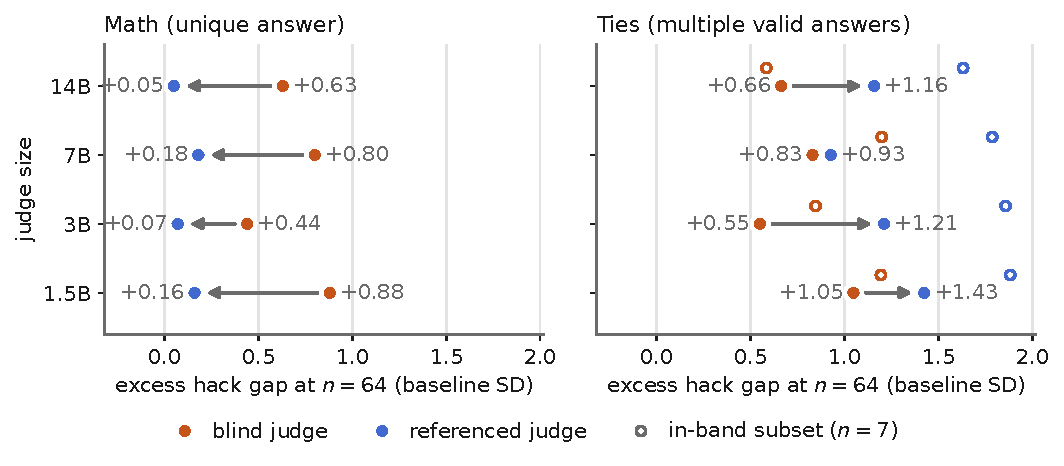
\includegraphics[width=\textwidth]{figures/fig_inversion.pdf}
\caption{\textbf{The inversion.}
Excess hack gap at $n{=}64$ for blind (orange) and referenced (blue) judges at four Qwen2.5 judge scales; arrows show the effect of adding the reference.
Left: unique-answer math (companion A~\cite{companionA}), where the reference collapses the gap $4$--$13\times$ at every scale.
Right: \textsc{RewardBench-2} Ties generation tasks with multiple valid answers ($n{=}51$ items), where the reference \emph{raises} the gap at every scale; small hollow markers show the registered in-band subset ($n{=}7$ items), which agrees in direction at every scale.
\textbf{Takeaway: the same trusted reference that collapses gaming on unique-answer tasks increases it when several answers are valid.}}
\label{fig:inversion}
\end{figure}

The answer is an inversion, and the mechanism behind it is directly manipulable.
At all four judge scales the referenced judge inflates the scoreboard more than its blind twin, with oracle regret directionally worse as well (Figure~\ref{fig:inversion}, Table~\ref{tab:fullset}).
The mechanism is anchoring, and rotating the reference proves it causal: re-judging the same frozen pools with the reference switched to a different valid answer raises the score of the identical sample text by $+3.1$ to $+9.5$ points on a 0--10 scale when the new reference matches it, every CI excluding zero ($n{=}40$ items per cell), so the premium follows the shown reference rather than any property of the answer (Figure~\ref{fig:anchoring}).
Combined with companion A's capability gate on code, the two results yield a two-condition boundary, which we offer as a conditional finding rather than a law: a reference helps if and only if the answer is effectively unique and the judge can verify against it.

\section{Setup}
\label{sec:setup}

\paragraph{Tasks.}
We built 51 generation tasks from \textsc{RewardBench-2} Ties items~\cite{malik2025rewardbench2}, each with at least two enumerated valid answers.
Each task stores the full valid set, which serves as the oracle, and one seeded-random member of that set designated at build time as the reference (\texttt{ref\_answer}) shown in the judge's referenced condition.
The prompts ask for exactly the kind of answer the valid set enumerates (short factual or constrained responses admitting several correct values).

\paragraph{Generation and oracle.}
Qwen2.5-7B-Instruct writes 64 samples per task at temperature 1.0, identical to the math and code protocol of companion A.
The oracle extracts the boxed answer (falling back to the whole reply) and checks loose-normalized membership in the enumerated valid set.
Correct therefore means ``any valid answer,'' never ``the reference.''

\paragraph{Judges.}
The judge ladder is Qwen2.5 Instruct at 1.5B, 3B, 7B, and 14B, each run blind (no reference) and referenced (the stored \texttt{ref\_answer} in context), each under two rubric paraphrases $\{a, b\}$.
Selection uses rubric $a$ and reporting uses rubric $b$, which cancels winner's-curse inflation, exactly as in companion A.

\paragraph{Estimands.}
The \emph{excess hack gap} measures scoreboard inflation of the selected sample relative to true quality, in baseline standard deviations over a within-oracle-stratum permutation null (judge scores permuted among samples with the same oracle verdict).
\emph{Oracle regret} measures accuracy left on the table against best-possible selection.
Both estimators are the pre-registered ones from companion A, unchanged (\texttt{scripts/bon\_analysis.py}).

\paragraph{Registration, and one deviation from it.}
The design and three predictions were committed to the repository (commit \texttt{99c40ea}, 2026-08-22) before any generation, oracle scoring, or judge scoring.
\textbf{P-T1} (primary): the reference does not reduce oracle regret on multi-valid items; directionally it hurts selection quality, in contrast to math where the same contrast was strongly positive ($0.448 \to 0.010$ regret at 1.5B).
\textbf{P-T2} (mechanism): among oracle-valid samples, referenced judges score reference-matching samples above equally valid non-matching samples, and blind judges show a near-zero margin.
\textbf{P-T3}: the excess hack gap under the reference is not reduced relative to blind.
The registration committed a single analysis population: items with pool pass rate in $[0.2, 0.8]$, the in-band filter carried over from the math and code protocol; it did not pre-declare a full-pool analysis, in the appendix or anywhere else.
On this pool the filter left $n{=}7$ items, too few to power the primary contrast, so we adopted the full 51-item analysis post hoc, for power.
This is a deviation from the registration.
We report both analyses in Section~\ref{sec:rq1}: the full-pool deviation carries the headline numbers, and the registered in-band primary, though underpowered, agrees or ties with it in direction at every judge size.
A follow-up reference-rotation rerun (prediction \textbf{P-T2r}) was registered in an addendum after the primary analysis and before any re-judging: the same frozen 64-sample pools are re-judged with \texttt{ref\_answer} rotated by a seeded permutation to a different member of each item's valid set, with generation and oracle scoring unchanged.
Its results are reported in Section~\ref{sec:rq2}.

\section{Results}

\subsection{RQ1: Does the reference help under selection pressure? No: it inverts.}
\label{sec:rq1}

\begin{table}[t]
\centering
\small
\begin{tabular}{lcccccc}
\toprule
& \multicolumn{2}{c}{Excess hack gap ($\sigma$)} & \multicolumn{2}{c}{Oracle regret} & \multicolumn{2}{c}{Paired $\Delta$gap (ref $-$ noref)} \\
\cmidrule(lr){2-3} \cmidrule(lr){4-5} \cmidrule(lr){6-7}
Judge & blind & ref & blind & ref & $\Delta$ & 95\% CI \\
\midrule
1.5B & $+1.05$ & $+1.41$ & $0.137$ & $0.157$ & $+0.35$ & $[-0.11, 0.79]$ \\
3B   & $+0.55$ & $+1.22$ & $0.137$ & $0.157$ & $+0.65$ & $[-0.03, 1.35]$ \\
7B   & $+0.82$ & $+0.91$ & $0.118$ & $0.137$ & $+0.08$ & $[-0.49, 0.61]$ \\
14B  & $+0.67$ & $+1.15$ & $0.078$ & $0.098$ & $+0.47$ & $[-0.21, 1.19]$ \\
\midrule
\multicolumn{5}{l}{Pooled item-level $\Delta$gap (4 scales averaged, cluster bootstrap)} & $+0.39$ & $[+0.04, +0.75]$ \\
\bottomrule
\end{tabular}
\caption{\textbf{Best-of-64 on 51 multi-valid Ties tasks (full-pool analysis; post-hoc deviation from the registered in-band filter, adopted for power).}
Excess hack gap (baseline SD over the within-oracle-stratum permutation null) and oracle regret per judge scale and condition, with paired item-level ref-minus-noref gap deltas and bootstrap CIs.
The reference worsens both readouts directionally on every row; per-scale gap deltas do not individually reach significance at $n{=}51$, the pooled gap delta does, and the regret deltas ($+0.020$ per scale, pooled $+0.020$ $[-0.025, +0.069]$) all cross zero.
\textbf{Takeaway: adding the reference never helps, directionally hurts on every row, and the pooled gap inflation excludes zero.}}
\label{tab:fullset}
\end{table}

Both registered outcome predictions hold directionally at every judge scale, with the gap carrying the significant evidence and the regret consistent but weaker.
P-T1 held directionally: oracle regret is higher under the reference at every scale, $0.137 \to 0.157$ at 1.5B and at 3B, $0.118 \to 0.137$ at 7B, and $0.078 \to 0.098$ at 14B, so the reference never buys back selection quality.
The regret deltas are small, however: each per-scale delta is $+0.020$ with a bootstrap CI crossing zero (for example $[-0.039, +0.078]$ at 1.5B), and the pooled regret delta is $+0.020$ $[-0.025, +0.069]$, so the regret evidence is directionally consistent but not individually significant, and we do not lean on it.
P-T3 held: the excess hack gap is higher under the reference at all four scales, $+1.05 \to +1.41$ at 1.5B, $+0.55 \to +1.22$ at 3B, $+0.82 \to +0.91$ at 7B, and $+0.67 \to +1.15$ at 14B (Table~\ref{tab:fullset}).

The paired item-level gap deltas are positive at all four scales ($+0.35$, $+0.65$, $+0.08$, $+0.47$) but each per-scale 95\% CI crosses zero at $n{=}51$ items.
Pooling across scales gives a significant effect: a cluster bootstrap that resamples the 51 items and, for each item, averages the four scales' per-item ref-minus-blind gap deltas yields $+0.39$ $[+0.04, +0.75]$, a CI excluding zero (Table~\ref{tab:fullset}, bottom row).
The four judge scales share items and a generator, so they are not independent replications; the pooled estimator treats scale as a fixed effect and items as the sole resampling unit, and it upgrades the dynamic claim from directional to significant at the pooled level, not to four separately significant replications.
What carries the inference is the conjunction of the individually significant pieces: the pooled item-level gap delta of $+0.39$ $[+0.04, +0.75]$, the conditional selection collapse of Section~\ref{sec:rq2} ($90$--$100\%$ referenced versus $70\%$ blind), the causal anchoring effect under reference rotation (paired same-sample deltas and cross-sectional margins, every CI excluding zero), and an opposite-signed effect of the same lever on math measured with identical estimators.
The regret deltas and the per-scale gap deltas are directionally consistent supporting evidence, not standalone results.

The registered primary analysis agrees or ties in direction at every size.
On the $n{=}7$ in-band items that survive the registered $[0.2, 0.8]$ filter, the referenced gap exceeds the blind gap at all four sizes ($+1.19 \to +1.88$ at 1.5B, $+0.90 \to +1.89$ at 3B, $+1.22 \to +1.74$ at 7B, $+0.53 \to +1.58$ at 14B), and referenced regret is worse at three of four sizes ($0.14 \to 0.43$ at 1.5B, $0.43 \to 0.57$ at 3B, $0.43 \to 0.57$ at 7B, and a tie at $0.29$ at 14B).
Seven items support no significance claim, but the analysis the registration actually committed points the same way as the full-pool deviation on every row (hollow markers in Figure~\ref{fig:inversion}).

The contrast with unique-answer math is the point.
On math the identical protocol gives blind gaps of $+0.88/+0.44/+0.80/+0.63$ collapsing to $+0.16/+0.07/+0.18/+0.05$ with the reference, a $4$--$13\times$ reduction at every scale~\cite{companionA}.
The same lever, the same judges, the same estimators, and the sign flips with the task's answer structure (Figure~\ref{fig:inversion}).

\subsection{RQ2: Why? The judge stops grading validity and starts grading proximity, and rotating the reference proves it.}
\label{sec:rq2}

\begin{figure}[t]
\centering
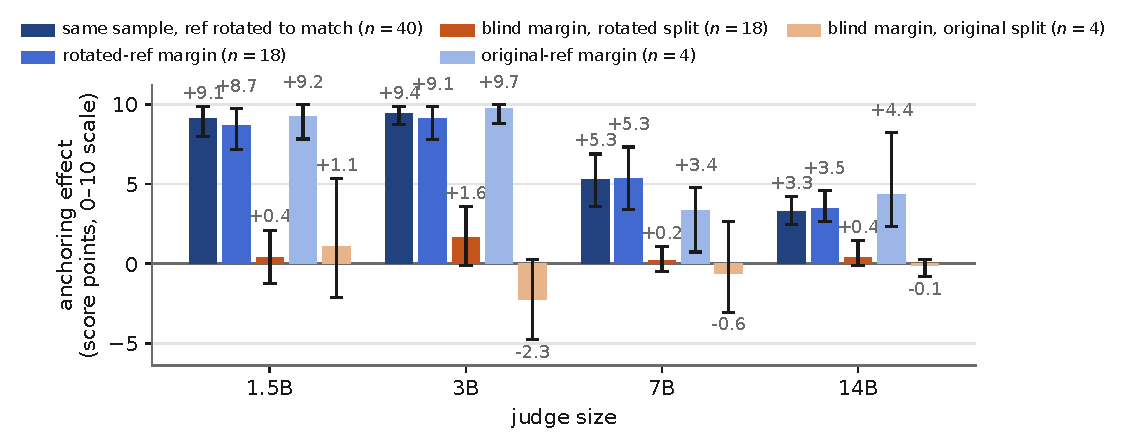
\includegraphics[width=0.88\textwidth]{figures/fig_anchoring.pdf}
\caption{\textbf{Takeaway: the anchoring premium follows whichever valid answer is shown as the reference, moving with the reference even for identical sample text; blind judges pay no premium.}
Anchoring effects (0--10 score scale) per judge scale, averaged over the two rubric paraphrases; whiskers span the union of the two paraphrases' 95\% bootstrap CIs.
Navy: paired same-sample deltas, the score gain of the identical sample when the reference is rotated to match it ($n{=}40$ items per cell).
Blue: cross-sectional margin of valid matching over valid non-matching samples in the rotation arm ($n{=}18$).
Light blue: the same margin in the original-reference arm ($n{=}4$).
Orange: blind judges scored on the same split as a placebo ($n{=}4$).}
\label{fig:anchoring}
\end{figure}

P-T2 and its registered follow-up P-T2r both held, and the rotation intervention turns the mechanism claim from an association into a causal one.
The rotation arm intervenes on the only variable the mechanism claim is about: the same 51 items, the same frozen 64-sample pools, the same oracle labels, but \texttt{ref\_answer} rotated by a seeded permutation to a \emph{different} member of each item's valid set, registered before any re-judging (Section~\ref{sec:setup}).
If the judge graded answer quality, a sample's score would not depend on which valid answer sits in the reference slot; if the judge anchors, the score must follow the shown reference.

The strongest readout is within-unit and paired: the identical sample text, scored twice.
For every oracle-valid sample whose answer matches the rotated reference but not the original, we pair its judge score across the two runs, same item, same rubric, nothing changed but the reference.
The score of the identical sample rises by $+9.48$ $[+8.95, +9.84]$ at 1.5B, $+9.28$ $[+8.70, +9.70]$ at 3B, $+4.57$ $[+3.62, +5.52]$ at 7B, and $+3.07$ $[+2.47, +3.71]$ at 14B under rubric $a$, with rubric $b$ replicating at $+8.73$, $+9.58$, $+5.96$, and $+3.47$ ($n{=}40$ items per cell, every CI excluding zero; Figure~\ref{fig:anchoring}, navy bars).
Nothing about the answer changed, so the premium is caused by the reference, full stop.
The effect is monotone in judge scale: near-total at 1.5B and 3B, where the delta saturates the 10-point scale, roughly half the scale at 7B, and a third of it at 14B.
More capable judges anchor less, but none stop.

The cross-sectional view corroborates.
Among oracle-valid samples we compute the within-item margin: mean judge score of samples matching the designated reference minus mean score of valid samples that do not match, with blind judges scored on the same split as a placebo, since they never see the reference.
Rotation puts valid matching and valid non-matching samples in coexistence on $n{=}18$ items per cell, up from 4 in the original arm, and the referenced margin toward the newly designated answer is $+9.00$ $[+7.95, +9.74]$ at 1.5B, $+9.05$ $[+7.81, +9.85]$ at 3B, $+4.75$ $[+3.39, +6.19]$ at 7B, and $+3.26$ $[+2.64, +3.92]$ at 14B under rubric $a$, with rubric $b$ replicating at $+8.36$, $+9.12$, $+5.93$, and $+3.67$.
Every CI excludes zero, the same monotone scale trend holds, and because the answers boosted under rotation are exactly the answers buried in the original arm, the margin is a property of what the judge is shown, not of the answers themselves.

The original-reference arm agrees, with an honest caveat on its size.
That arm has only $n{=}4$ items where both sample types coexist, because of the 10 items whose pool contains a valid reference-matching sample, 6 have zero other-valid samples (all 64 samples give the same answer), a property of the generator's answer distribution.
On those 4 items the referenced margin is $+2.6$ to $+9.99$ with all eight referenced cells excluding zero, and the extreme 3B rubric-$b$ cell ($+9.99$ $[+9.98, +10.0]$) is ceiling-limited by score saturation rather than precisely estimated.
Blind judges show nothing of the kind in either arm: no blind cell has a positive margin distinguishable from zero; seven of eight straddle zero, and the one blind cell excluding zero is negative ($-2.5$ $[-4.7, -0.2]$ at 3B, rubric $b$), roughly the one boundary exclusion expected by chance among 16 cells tested at the 95\% level.

The margin translates into near-deterministic selection.
Conditional on the sampled pool containing at least one sample whose answer matches the shown reference, which happens on 10 of the 51 items, referenced judges select a reference-matching sample $10/10$, $10/10$, $9/10$, and $10/10$ times at 1.5B, 3B, 7B, and 14B, versus $7/10$ for the blind judge at every size.
Whenever the reference-matching answer is on offer, the referenced judge takes it $90$--$100\%$ of the time; the $n{=}10$ base makes this a mode-collapse observation rather than a precise rate.

The margin also explains the inversion rather than merely accompanying it: a judge that boosts one valid answer and buries the rest turns best-of-64 into a lottery over reference proximity.
That lottery inflates reported scores relative to true quality (the gap, significantly) while directionally degrading the chance of selecting a correct answer (the regret), which is exactly the pattern of Table~\ref{tab:fullset}.

\subsection{RQ3: Reconciling with unique-answer domains: a two-condition boundary.}

The two faces of the lever are one mechanism under two answer structures.
When the valid set has a single member, proximity to the reference and correctness are the same criterion, so anchoring is verification and the reference works as a checkable certificate: gaps collapse $4$--$13\times$ on math.
When the valid set has several members, proximity and correctness dissociate, the judge keeps anchoring anyway (Figure~\ref{fig:anchoring}), and the reference manufactures a systematic scoring error that selection pressure then exploits.
The static and dynamic results agree in sign, which the registration explicitly flagged as the informative outcome: the $7$--$8$ point static verdict cost~\cite{companionA} and the dynamic gap increase are the same anchoring channel read out two ways.

Capability is the second condition, and it is independent of multiplicity.
Companion A found that on code, where using the reference means mentally executing a test suite, a 1.5B judge gains nothing from the reference while 3B and above collapse their gaps; the reference only helps judges capable of verifying against it~\cite{companionA}.
Together the two results give a practitioner's rule, which we state as a conditional finding rather than a law, since it rests on one task family and one judge family so far: \emph{a trusted reference helps if and only if (i) the task's answer is effectively unique, and (ii) the judge can verify a candidate against it}.
Fail condition (ii) and the reference is inert.
Fail condition (i) and the reference is actively harmful, statically and under optimization pressure, at every judge scale we tested.
More capable judges reduce the anchoring premium but do not eliminate it.
The operational advice is correspondingly simple: before installing a reference, ask whether a correct answer different from the reference exists; if yes, either enumerate the valid set and check membership, as our oracle does, or leave the judge blind.

\subsection{Registered next test: synthetic multiplicity, dose and mitigation.}

The Ties pool fixes neither the number of valid answers nor the model families, so the boundary statement above is a conjecture awaiting a sharper test, and we have registered that test before running it.
The design constructs synthetic tasks with exactly $k$ valid answers, $k \in \{1, 2, 4, 8, 16\}$, giving a dose-response curve in multiplicity with the $k{=}1$ control inside the same design.
Two registered mitigation arms modify only the judge's context: an instruction stating that the reference is one valid answer among many, and showing $\min(3, k)$ references.
The judge set includes cross-family models (Llama-3.1-8B, phi-4) and the generator is a Llama model, breaking the shared-family structure of the present ladder.
Predictions P-S1 through P-S5 were committed before any generation (repository commit \texttt{c505c23}).
No results from this design are claimed here.

\section{Limitations}

The task pool is small and single-sourced.
All dynamic results rest on 51 Ties-derived items; the per-scale paired gap deltas individually cross zero at this $n$, and only the pooled item-level delta ($+0.39$ $[+0.04, +0.75]$) excludes zero.
The regret deltas are directionally consistent but never individually significant: $+0.020$ at every scale with all CIs crossing zero, pooled $+0.020$ $[-0.025, +0.069]$, so the selection-quality half of P-T1 is supported in direction only.
The four-scale directional agreement has a sign-test floor of $p = 1/16$, the best attainable with four paired observations, and the four judge scales share items and a generator, so the pooled estimate treats scale as a fixed effect rather than as independent replications.
One generator (Qwen2.5-7B-Instruct) produced every candidate pool, so generator-specific answer distributions could modulate the dynamic effect sizes; the same distribution is what starved the original-arm margin analysis, since 6 of the 10 items with a valid reference-matching sample have no other valid answer among all 64 samples.
That original anchoring arm therefore rests on 4 items, and the conditional selection-collapse rates on 10; the registered rotation rerun repowered the mechanism to $n{=}18$ items per cell for the cross-sectional margin and $n{=}40$ for the paired same-sample deltas, but the collapse rates remain a 10-item observation.
The oracle is loose-normalized membership in an enumerated valid set; answers valid in substance but outside the enumeration, or normalization misses, would be scored as failures for every condition alike.
The analysis population is a registered/actual mismatch: the registration committed only the in-band $[0.2, 0.8]$ filter, which left $n{=}7$ items, and the full-pool analysis reported as primary here is a post-hoc deviation adopted for power, with the registered in-band analysis agreeing or tying in direction at every size (Section~\ref{sec:rq1}).
Finally, the generator and all four judges share the Qwen2.5 family, so family-specific answer styles or scoring habits could inflate or deflate the ladder-level effect sizes, and the scale trend in the anchoring effect should be read as within-family.
The rotation intervention is immune to this confound, since it compares the same judge on the same samples and varies only the shown reference, but the dynamic inversion is not; cross-family replication with a Llama generator and Llama/phi judges is registered as predictions P-S4 and P-S5 of the synthetic-multiplicity design.

\section{Related work}

Reference-guided judging is standard practice with documented benefits on unique-answer tasks.
\textsc{MT-Bench} popularized providing a reference for math and reasoning grading~\cite{zheng2023judging}, reference-guided verdicts raise human agreement on QA~\cite{refguided2024}, and letting the judge first produce its own answer as a self-reference helps similarly~\cite{dobefore2025}.
The complementary failure is also documented: without any reference, judges drift generous~\cite{generous2026}.
Our results do not contradict this literature; they bound it, locating its validity in the unique-answer regime.

The static half of the failure is prior art, and we position this paper accordingly.
Solution Fixation Bias shows that LLM judges penalize valid solutions that differ from the provided reference in a static pairwise setting~\cite{fixation2025}, reference-guided evaluation is reported to degrade on open-ended tasks~\cite{judgingref2026}, and our companion audit found the same $7$--$8$ point Ties cost for references of any authorship~\cite{companionA}.
We claim none of that as new.
What this paper adds is the dynamic result, the inversion under best-of-$n$ selection pressure with excess-gap and collapse estimands; the causal mechanism, anchoring demonstrated by reference rotation rather than inferred from static error rates; predictions committed before data (\texttt{registration.md}, git-timestamped); and the boundary statement, help if and only if the answer is effectively unique and verification is within judge capability, with the $k{=}1$ control registered inside the same synthetic-multiplicity design.
The anchoring result also bears on a recommended practice: having the judge generate its own reference before grading~\cite{dobefore2025} is contraindicated on multi-valid tasks, since the static any-author result shows self-generated references anchor just as external ones do.

\textsc{RewardBench-2} supplies the multi-valid substrate.
Its Ties subset was built precisely because equally valid answers expose evaluator brittleness~\cite{malik2025rewardbench2}; we convert those comparisons into generation tasks with enumerable oracles and put them under selection pressure.
Optimization against imperfect evaluators is the classic overoptimization setting~\cite{gao2022scaling}; our contribution is to show that a mitigation assumed to reduce exploitability can increase it, depending on answer structure.
Companion A establishes the unique-answer collapse, the capability gate, and the static Ties result this paper extends dynamically~\cite{companionA}; companion B gives the underlying decomposition, that comparison-to-reference metrics measure properties of the reference rather than of the solution~\cite{companionB}.

\medskip
\noindent\textbf{Conclusion.}
The reference lever is not a safety default; it is a conditional instrument with a sign.
Unique answer and a capable judge: it collapses gaming.
Multiple valid answers: it becomes the attack surface, and the judge's trust in the answer key is exactly what gets exploited.

\bibliographystyle{plain}
\bibliography{references}

\end{document}
